\documentclass[a4paper,10pt,notitlepage,twocolumn,oneside]{article}

%\documentclass[prl]{revtex4}%Format for Phys. Rev. Lett. and other APS journals


  %%%%%%%%%%%%
 % PACKAGES %
%%%%%%%%%%%%


% Additional math & symbols by the American Mathematical Society
\usepackage{amsmath}
\usepackage{amssymb}

% Support for various unit symbols
\usepackage[squaren]{SIunits}

% Use more of the paper
\usepackage{a4wide}

% Use T1 encoded fonts
\usepackage[T1]{fontenc}

% Multi language support
\usepackage[spanish,german]{babel}

% Latin1 input encoding support
\usepackage[latin1]{inputenc}

% "Times" as standard roman font
\usepackage{times}

% "Times" as standard roman font _and_ math roman as well
%\usepackage{mathptmx}

% Support for T1 encoding with standard computer modern fonts
%\usepackage{ae}

% Hyperlink references
\usepackage[dvips=true]{hyperref}

% Index support
\usepackage{makeidx}

% Fancy headers
\usepackage{fancyhdr}

% Extended graphics support
\usepackage{graphicx}

%\usepackage[dvips]{graphics}
% alter usepackage-Befehl

% Set space between lines
\usepackage{setspace}

% Text companion extended symbols
\usepackage{textcomp}





  %%%%%%%%%%%%
 % DOCUMENT %
%%%%%%%%%%%%

\begin{document}
\title{Title of Paper}
\author{V. Nachname$^{1,}$\thanks{Corresponding author. E-mail: email@email.de}\, Prof. Dr. V. Nachname$^1$\\
\emph{$^1$ Hochschule Darmstadt - University of Applied Sciences,
Haardtring 100}\\
\emph{64295 Darmstadt, Germany}
}

\date{\today} % autodate
%\date{19.10.2009}

\maketitle

%\keywords{Computergraphics, Stereoscopic, Interfaces}

\section*{Abstract}
test
Abstract text here\ldots

\section*{Introduction}

Introduction text here\ldots

\section*{Main part of the paper}

main text here\ldots



\section*{Conclusions}

Conclusion, summary and outlook\ldots

\begin{thebibliography}{99}

\bibitem{ANGELIDIS} Angelidis A., ans Neyret, F. 2005. Simulation of smoke based on vortex filament primitives. In ACM-SIGGRAPH/EG, Symposium on Computer Animation.

\bibitem{BASCOM} Bascom, W. 1980. Waves and Beaches. Anchor Books, Garden City, NY.

\end{thebibliography}


% \section*{TexStuffExample}


  %%%%%%%%%%%%%%%%
 % REGULAR TEXT %
%%%%%%%%%%%%%%%%

BLABLA\\
\emph{BLABLA}\\
BLABLA
BLABLA\\
BLABLA
BLABLA
\\
i'm a line with dots\ldots
\\




  %%%%%%%%%%%%
 % FORMULAS %
%%%%%%%%%%%%

Formulas
\[ a^2 + b^2 = c^2\]
\[ b = \sqrt{c^2 - a^2} \]

Pictures (Fig. \ref{fig:egPic})\\
\begin{figure}[htp]
\begin{center}
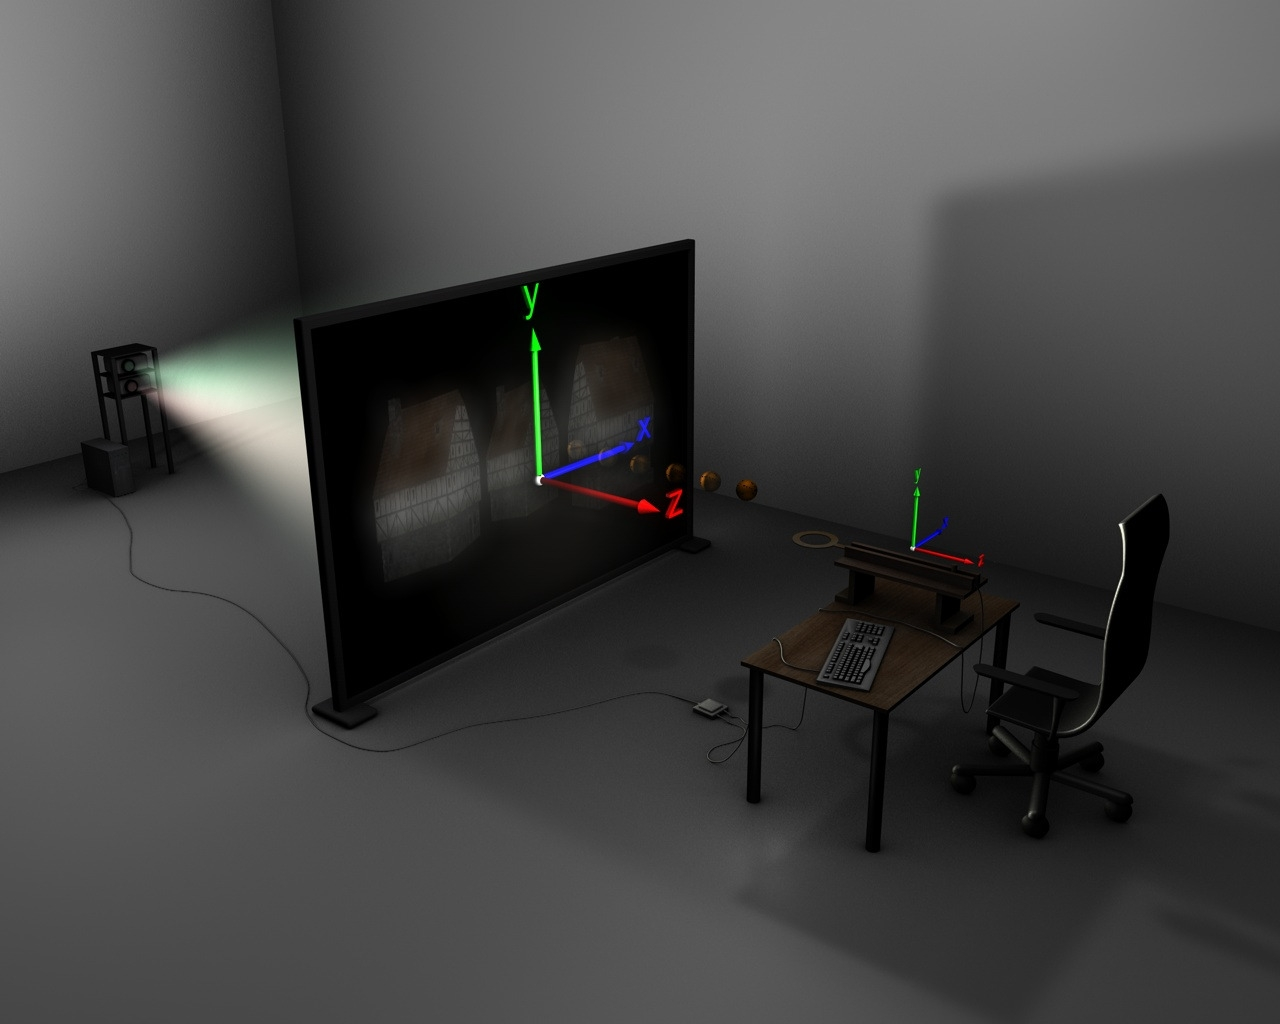
\includegraphics[width=6cm]{Pic/exampleimage.jpg}
\caption{description of the sketch}
\label{fig:egPic}
\end{center}
\end{figure}




  %%%%%%%%%%
 % TABLES %
%%%%%%%%%%

Tables (Tab. \ref{tab:mytable})\\
\begin{table}[htbp]
\begin{center}
\begin{tabular}{|l||c|c|c|} \hline
Name & Test 1 & Test 2 & Final \\ \hline \hline
Bob & 93 & 92 & 70 \\ \hline
John & 93 & 92 & 70 \\ \hline
Peter & 78 & 41 & 77 \\ \hline
Jack & 94 & 97 & 45 \\ \hline
Jane & 95 & 87 & 96 \\ \hline \hline
Avg: & 94 & 90 & 83 \\ \hline
\end{tabular}
\caption{\label{tab:mytable}This is a table with random numbers.}
\end{center}
\end{table}


 % how to use/include a table, formula, picture... 

\bibliography{bib}
\bibliographystyle{apalike}

\end{document}
